\documentclass{beamer}
\usepackage[orientation=portrait,size=a0,scale=1.4,debug]{beamerposter}
\mode<presentation>{\usetheme[articleid=WEPOPRPO22]{LNLS}}
\usepackage{chemformula}
\usepackage[utf8]{inputenc}
\usepackage[german, english]{babel} % required for rendering German special characters
\usepackage{siunitx} %pretty measurement unit rendering
\usepackage{hyperref} %enable hyperlink for urls
\usepackage{ragged2e}
\usepackage{calc}
\usepackage{datetime}
\newlength{\mylength}

\usepackage{array,booktabs,tabularx}
\newcolumntype{Z}{>{\centering\arraybackslash}X} % centered tabularx columns

\title{\huge High Level Applications for Sirius}
\author{\underline{I. Stevani}, N. Milas, X. R. Resende, L. N. P. Vilela}
\institute{Brazilian Synchrotron Light Laboratory (LNLS), Campinas, Brazil}
\date{\monthname \ \the\year}

\newlength{\abstractheight}
\setlength{\abstractheight}{10cm}

\newlength{\columnheight}
\setlength{\columnheight}{95cm}

\begin{document}
\begin{frame}
\begin{beamercolorbox}[center]{postercolumn}
	\begin{minipage}{\textwidth}
		\parbox[t][\abstractheight]{\textwidth}{
		\begin{myblock}{\textit{Abstract}}
			Has been decided that Sirius will use EPICS as its distributed control system and this year the development of its High Level Applications (HLAs) started. Three development frameworks were chosen for building these applications: CS-Studio, PyQt and Matlab Middle Layer (MML). Graphical user interfaces (GUI) and machine applications have already been designed and implemented for a few systems using CS-Studio and PyQt: slow orbit feedback, lifetime calculation and top-up injection. Specific Sirius data structures were added to the MML scripts in order to allow for EPICS communication through LabCA.
		\end{myblock}
	}\end{minipage}
\end{beamercolorbox}
\begin{columns}
	\begin{column}{0.45\textwidth}
		\begin{beamercolorbox}[center]{postercolumn}
			\begin{minipage}{.98\textwidth}  % tweaks the width, makes a new \textwidth
				\parbox[t][\columnheight]{\textwidth}{ % must be some better way to set the height, width and textwidth simultaneously
					\begin{myblock}{Application Environment}
						\begin{itemize}
							\item \textbf{Machine Applications:} EPICS servers used to compute beam dynamics algorithms such as lifetime calculation and slow orbit feedback. Since they communicate with hardware through other EPICS servers (IOCs), they can be interpreted as EPICS clients too.
							\item \textbf{IOCs:} Also EPICS servers, but their main purposes are to control and establish communication with hardwares such as power supplies and BPMs.
							\item \textbf{Client Applications:} EPICS clients built to control and monitor PVs.
						\end{itemize}
						\begin{figure}
							\centering
							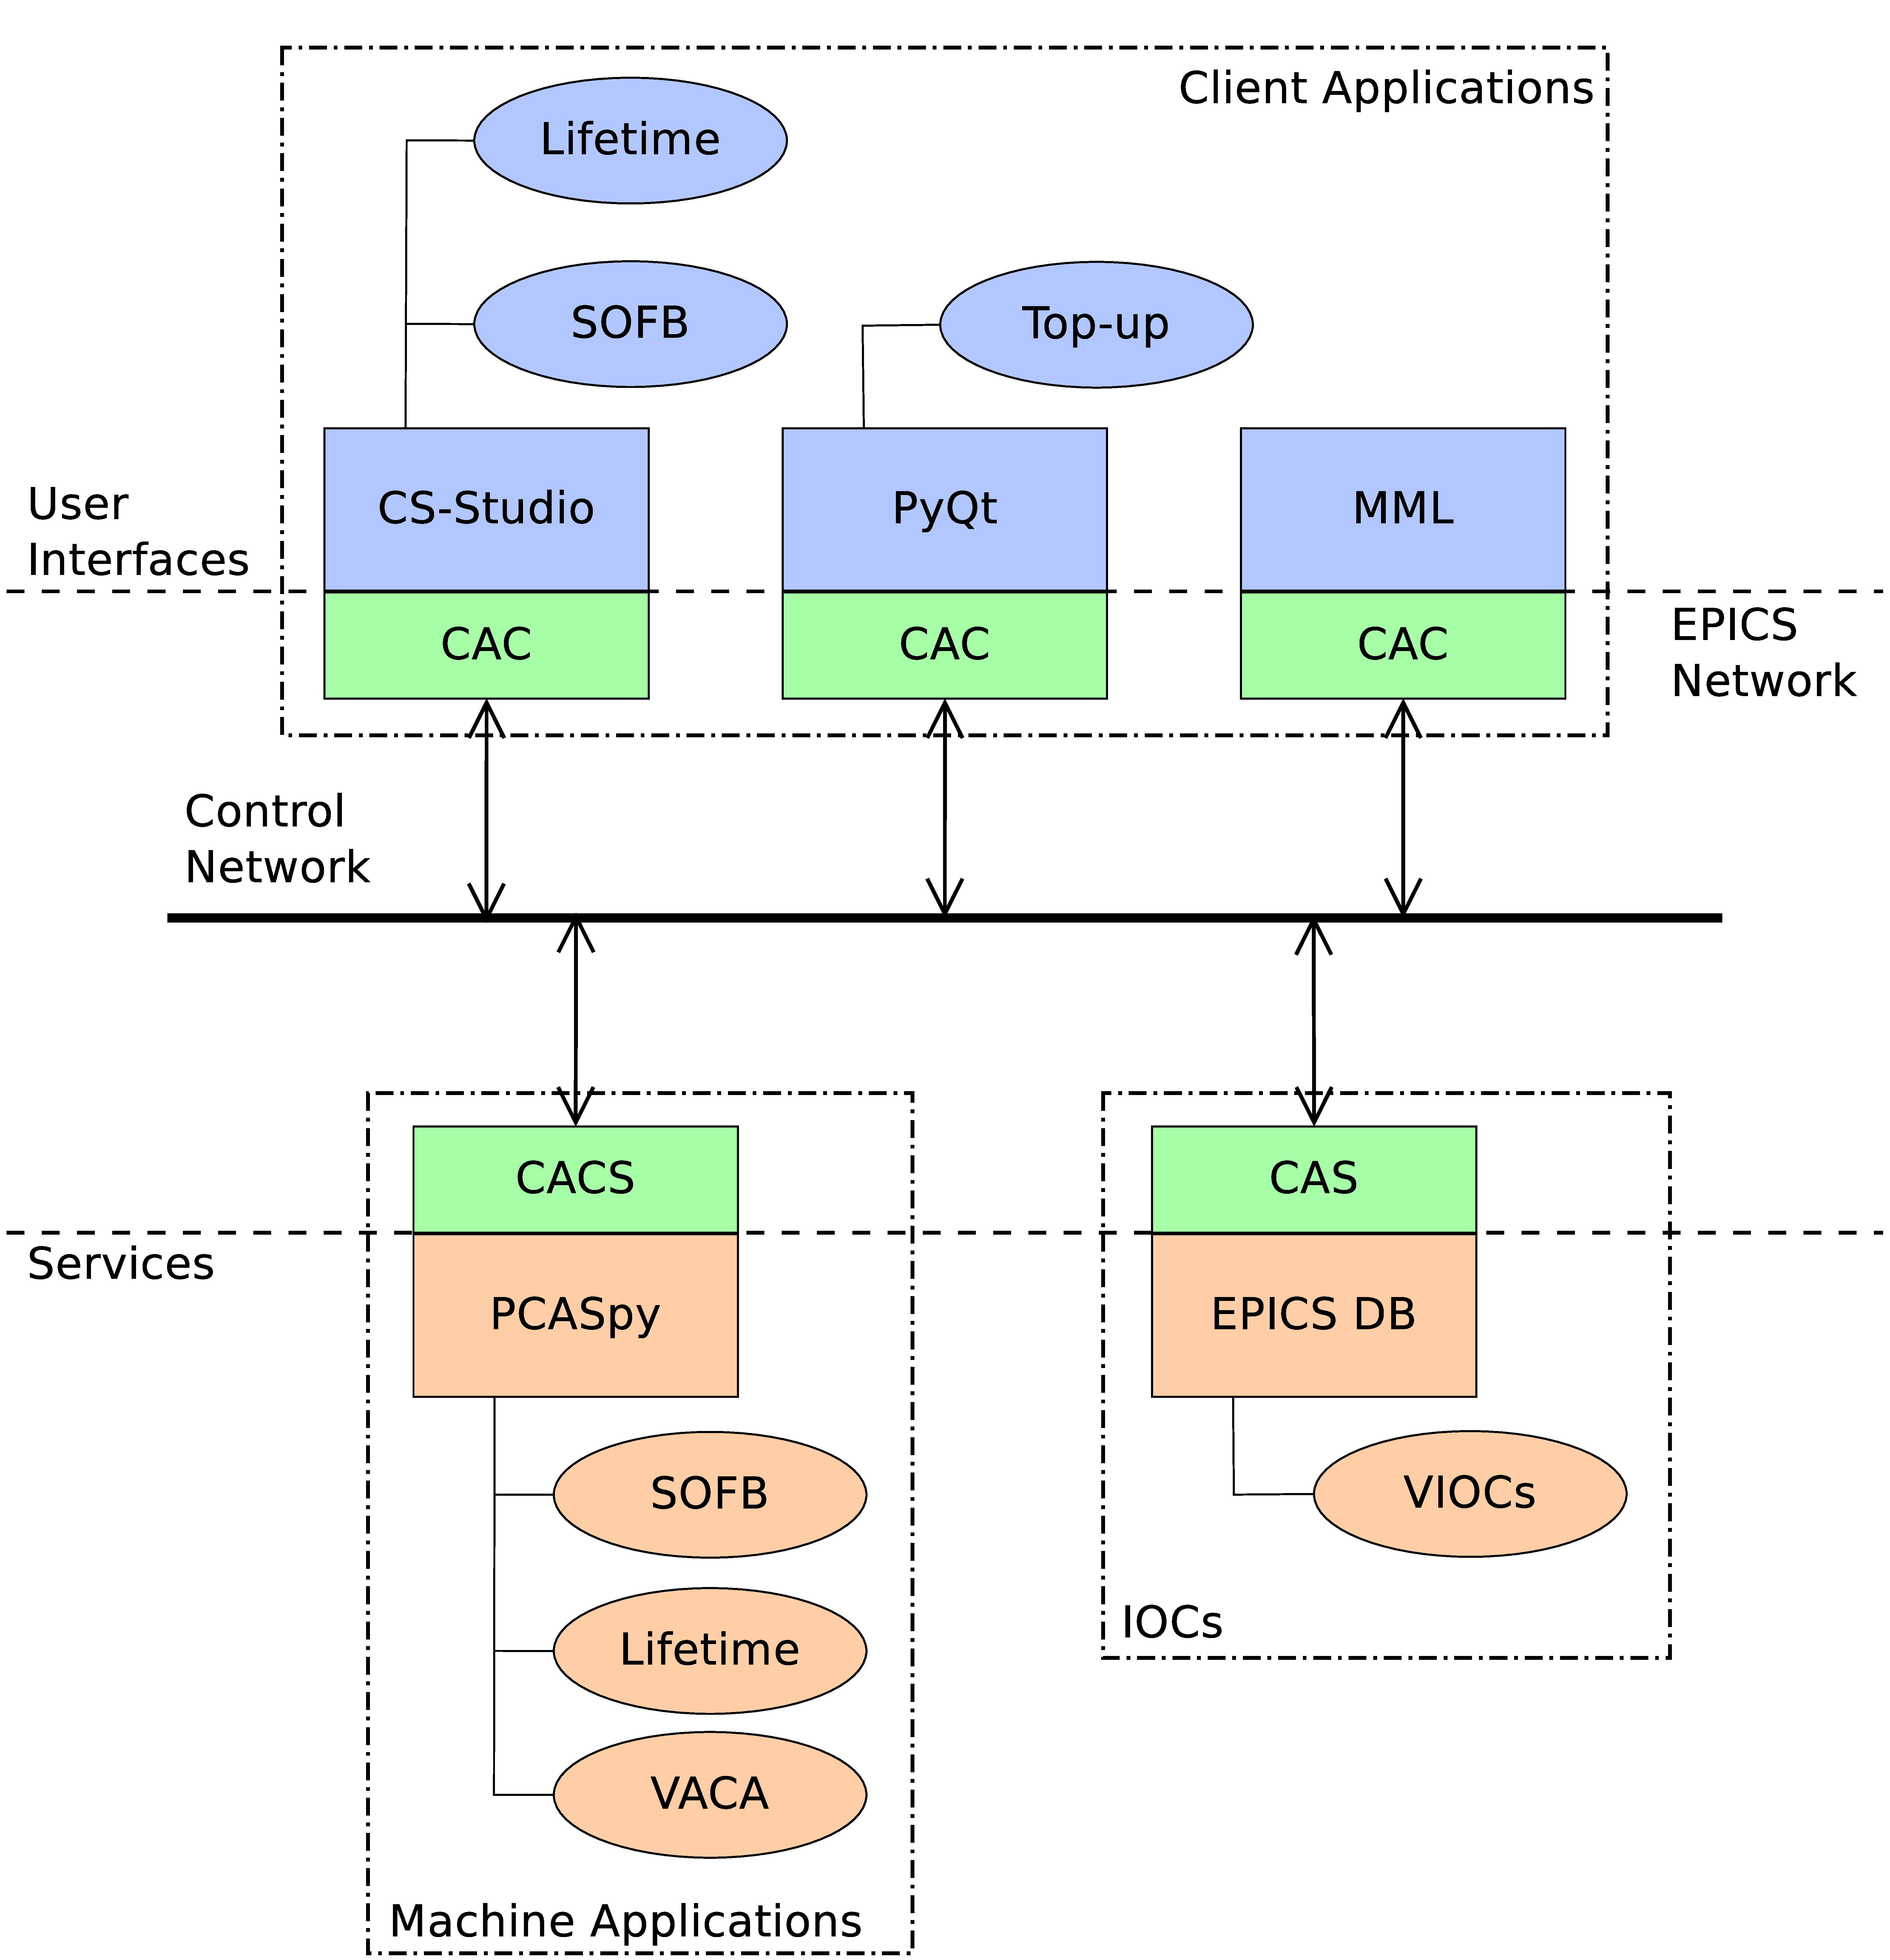
\includegraphics[width=0.85\textwidth]{../WEPOPRPO22f1.eps}
							\caption{Application environment schematic.}
						\end{figure}
					\end{myblock}
					\begin{myblock}{Top-up Injection}
						\textbf{Implemented functionalities}
						\begin{itemize}
							\item \textbf{Top-up Client Application:} Current and filling pattern display, injection mode selection, maximum current and maximum current decay adjustment.
						\end{itemize}
						\vspace{0.5cm}
						\begin{figure}
							\centering
							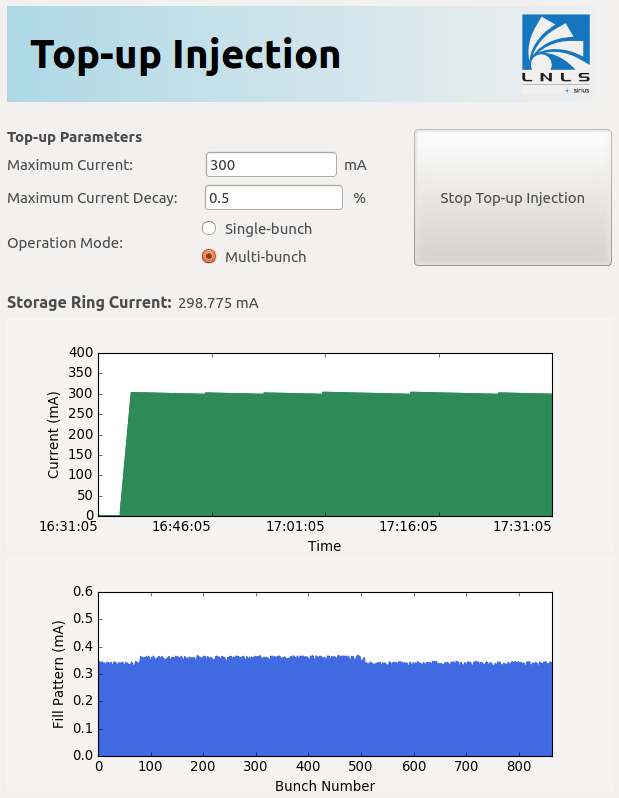
\includegraphics[width=0.684\textwidth]{../WEPOPRPO22f4.png}
							\caption{Top-up injection display application developed with PyQt.}
						\end{figure}
					\end{myblock}\vfill
		}\end{minipage}\end{beamercolorbox}
	\end{column}
	\begin{column}{.55\textwidth}
		\begin{beamercolorbox}[center]{postercolumn}
			\begin{minipage}{.98\textwidth} % tweaks the width, makes a new \textwidth
				\parbox[t][\columnheight]{\textwidth}{ % must be some better way to set the the height, width and textwidth simultaneously
					\begin{myblock}{Slow Orbit Feedback}
						\textbf{Implemented functionalities}
						\begin{itemize}
							\item \textbf{SOFB Machine Application:} Orbit/response matrix measurements and orbit corrections based on singular value decomposition (SVD), device selection, response matrix and reference orbit configurations, variable-size buffers with orbit data for averages, optional inclusion of RF frequency in the correction loop and corrector strength adjustments.
							\item \textbf{SOFB Client Application:} Plot displayed with measured orbit, widgets set for manual correction, the machine application mode selection and widgets for configuring sampling parameters for orbit average calculations.
						\end{itemize}
						\vspace{0.5cm}
						\begin{figure}
							\centering
							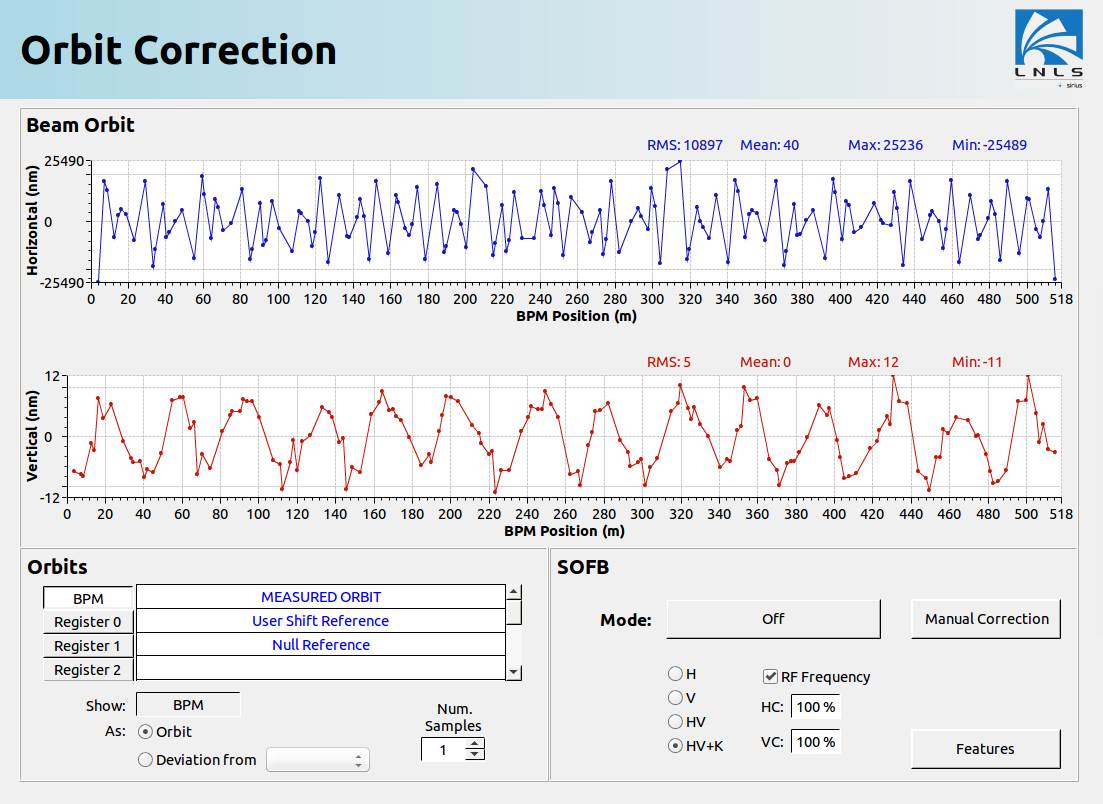
\includegraphics[width=0.85\textwidth]{../WEPOPRPO22f3.png}
							\caption{Orbit correction display application in the CS-Studio environment.}
						\end{figure}
					\end{myblock}\vfill
					\begin{myblock}{Lifetime Calculation}
						\textbf{Implemented functionalities}
						\begin{itemize}
							\item \textbf{Lifetime Machine Application:} Lifetime calculation and precision and sampling time input parameters.
							\item \textbf{Lifetime Client Application:} Current and lifetime display, lifetime unit selection, lifetime graphical display, algorithm parameters display and precision and sampling time adjustment.
						\end{itemize}
						\vspace{0.5cm}
						\begin{figure}
							\centering
							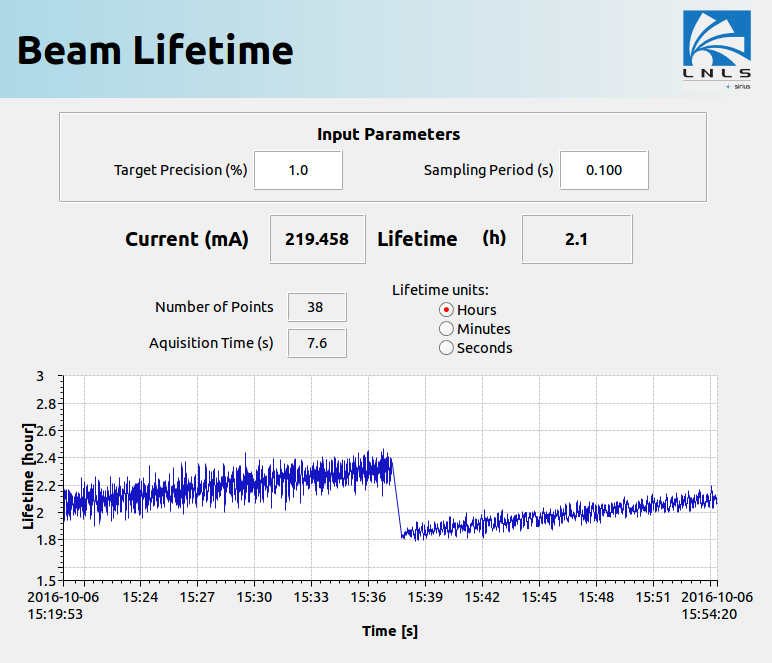
\includegraphics[width=0.85\textwidth]{../WEPOPRPO22f2.png}
							\caption{Lifetime display application in the CS-Studio environment.}
						\end{figure}
					\end{myblock}\vfill
		}\end{minipage}\end{beamercolorbox}
	\end{column}
\end{columns}
\end{frame}
\end{document}
